\section{Introduction}

In most real-world applications of object recognition, performance is time-sensitive and inherently tied to the many-class nature of the world.
In robotics, a small finite amount of processing power per unit time is all that is available for robust object detection if the robot is to usefully interact with humans.
In large-scale detection systems (e.g. image search), results need to be obtained quickly per image as the number of items to process is constantly growing.
In these cases, an acceptable answer at a reasonable time may be more valuable than the best answer given too late.

\begin{figure}[ht!]
\center{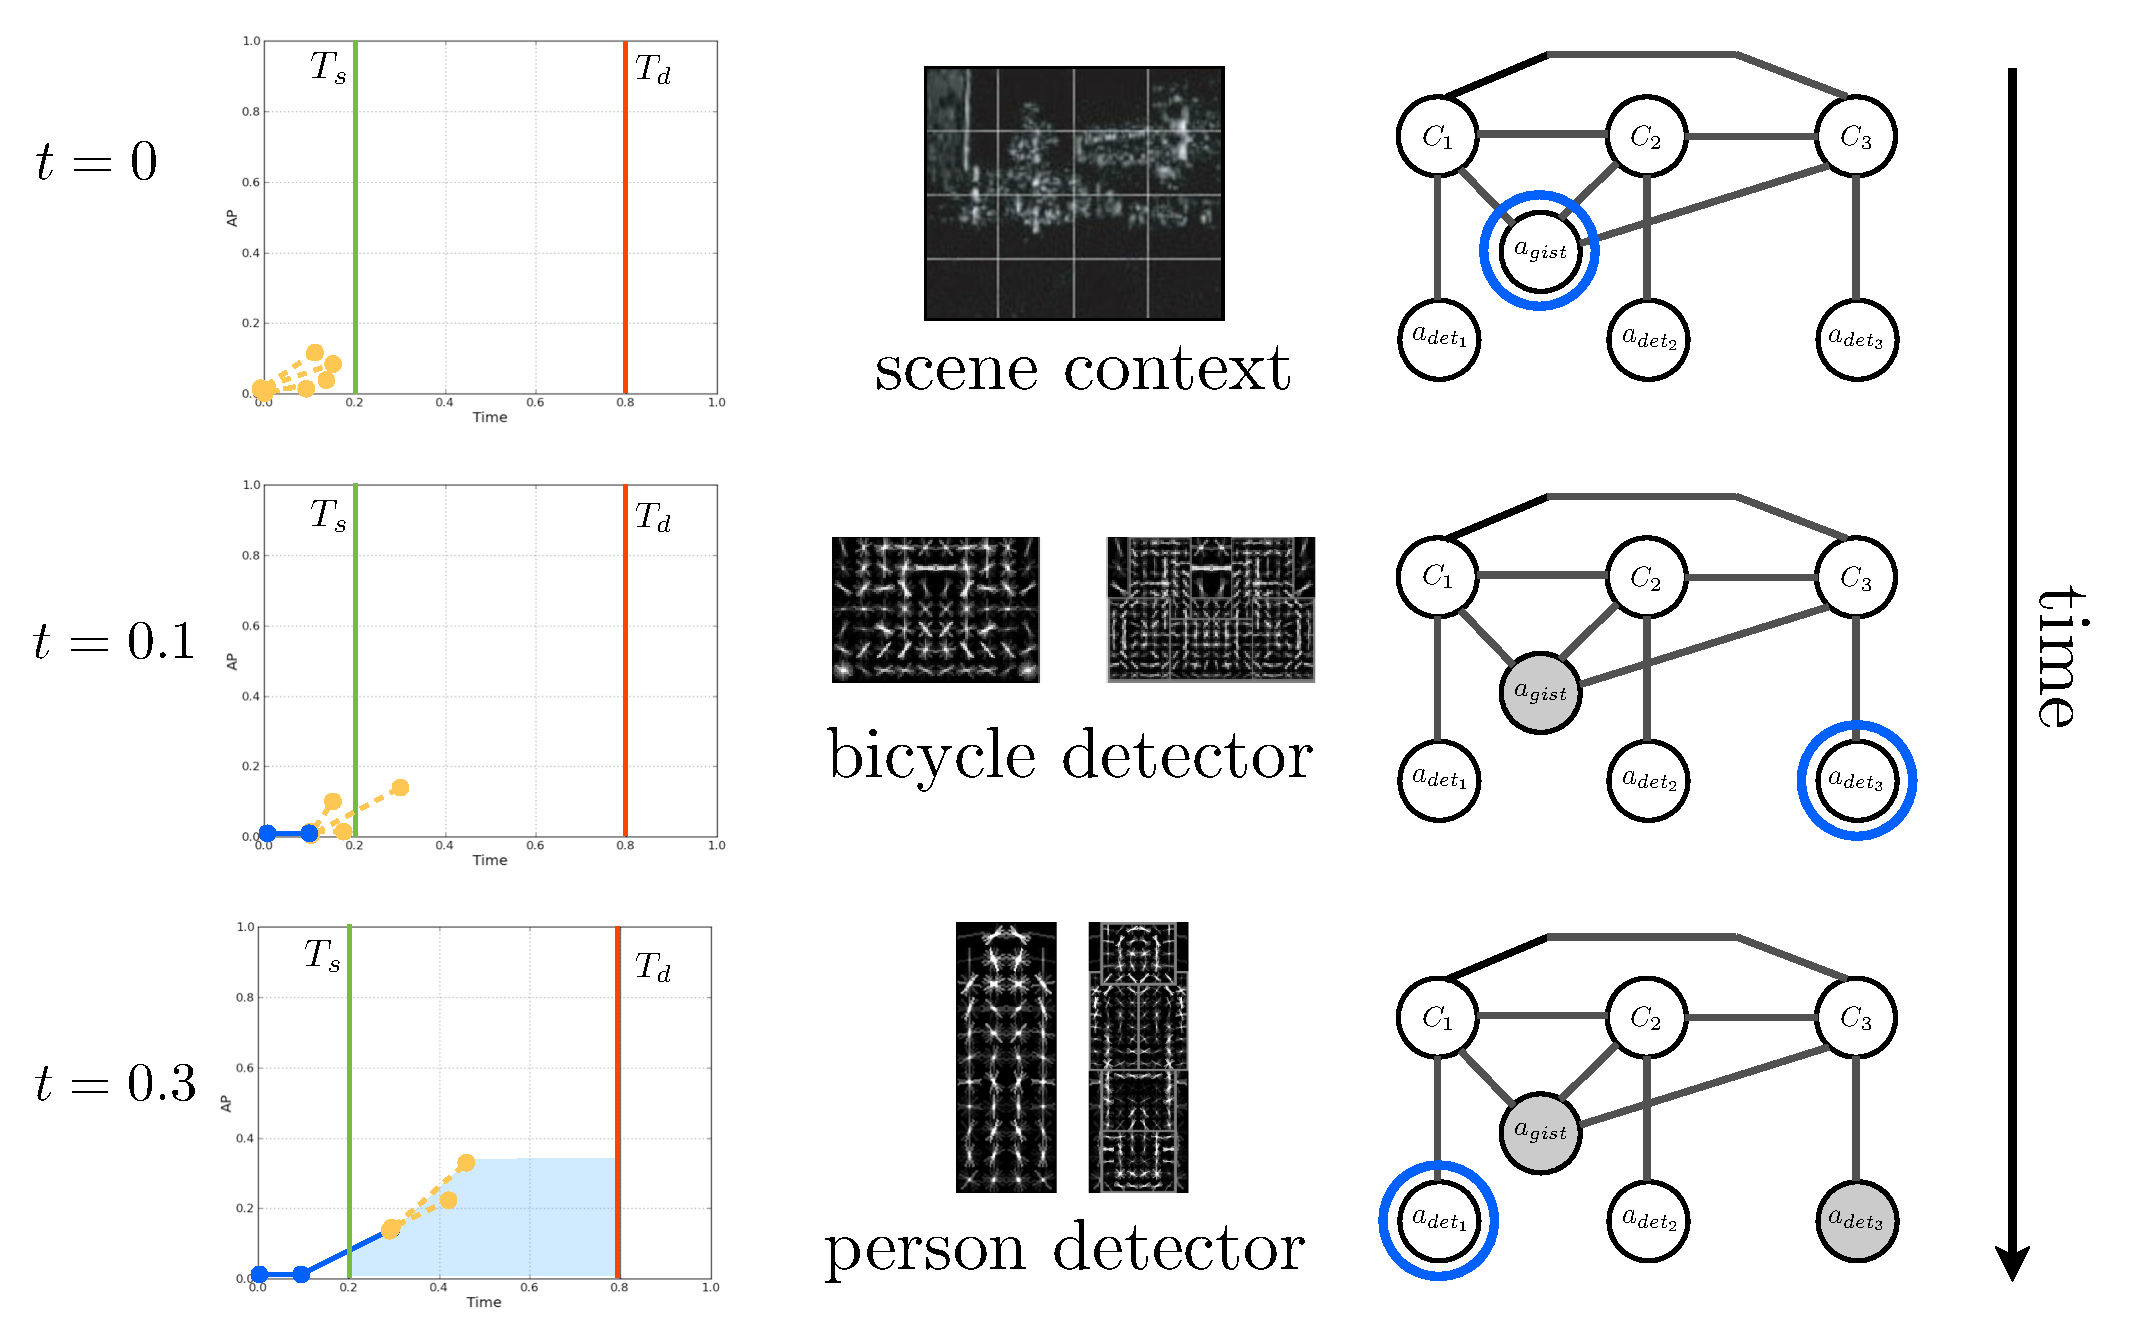
\includegraphics[width=0.86\linewidth]
    {../figures/figure1.pdf}}
  \caption{
A sample trace of our method.
At each time step beginning at $t=0$, potential actions are considered according to their \emph{value}, and the one with the highest value is picked.
The selected action is performed and returns observations, which influence the selection of the next action.
The final evaluation of a detection episode is the area of the AP vs. Time curve between the start and end times.
The value of an action is the expected value of the final evaluation if the action is taken and the policy continues to be followed, which allows actions without an immediate benefit to be scheduled.
}
  \label{fig:figure1}
\end{figure}

The conventional approach to evaluation of visual category recognition does not consider efficiency and evaluates performance independently across classes.
We argue that the key to tackling problems of dynamic recognition resource allocation is to start asking a new question:
\emph{What is the best performance we can get on a budget?}

We propose a new \emph{timeliness} measure of performance vs. time (shown in Figure~\ref{fig:figure1}), and present a method based on reinforcement learning that takes various detectors and classifiers as black boxes, and learns a dynamic policy for selecting detector and other actions to achieve the highest performance under this evaluation.
We are able to obtain better performance than baselines when there is less time available than is needed to exhaustively run all detectors.

A hypothetical system for vision-based advertising presents a case study.
The system will have different values and accuracies for objects of different classes, and the queue of unprocessed images will vary in size.
The detection strategy to maximize profit in such an environment has to be dynamic.
We explore this scenario using the PASCAL VOC datasets and evaluation regimes, and show that our learned dynamic policy offers a better strategy than a random or optimal static ordering of detectors.
